\documentclass[11pt]{article}
\usepackage{graphicx}
\usepackage{subfigure}
\usepackage{color}
\usepackage{rotating}
\usepackage{multirow}
\usepackage{setspace}
\usepackage{amsmath}
\usepackage{amssymb, amsfonts}
\usepackage{float}
\usepackage{verbatim}
%\usepackage[algo2e,ruled,vlined,linesnumbered]{algorithm2e}
%\usepackage{algorithm}
\usepackage{algorithmic}
\usepackage{multirow}
\usepackage[american]{babel}
\usepackage{dsfont}
%\usepackage{amsthm}
\usepackage{enumerate}

%\usepackage[latin1]{inputenc}
%\usepackage[T1]{fontenc}
\usepackage{eso-pic}
%\usepackage{latex8}
\usepackage{times}
\usepackage{hyperref}
\usepackage{breakurl}
\usepackage{tcolorbox}
\usepackage{geometry}

\geometry{letterpaper, total={8.5in,11in}, left=1.0in,  right=1.0in, top=1.0in, bottom=1.0in}


\usepackage{fancyhdr}
\pagestyle{fancy}
\fancyhf{}
\rhead{Risk of Death in Heart Failure Patients}
\lhead{}
\rfoot{Page \thepage}

\usepackage{indentfirst}

\begin{document}

\title{Risk of Death in Heart Failure Patients}
\author{Michael Pitts, Jasjeet Rangi, Albert Eo, Pranay Mittal, Arya Rajpal,
Nicholas Sulistio, Alison Wu}

%\date{\today}

\maketitle

\section{Introduction and Background}

{Heart failure/disease is the leading cause of death globally, accounting for 
around 16\% of the world’s total deaths. It occurs when the heart cannot pump 
enough blood to the body’s needs, causing  There are many factors that can play 
into death for people with heart failure such as smoking, diabetes, high blood 
pressure, and more. In this regard, it is important to know whether one is at 
high risk or low risk of death from heart failure based on these factors. 
Machine Learning can predict a patient’s risk/survival based on the features of 
the dataset of medical records.

With the help of a classification model, patients with heart failure will know 
if they are at high or low risk of death based on their values of clinical 
laboratory tests, conditions, and lifestyle habits. Depending on what the 
result is of the classification, patients may then look into changing some of 
their lifestyle habits to try to be of lower risk. This would be done by a 
follow-up appointment.}


\section{Literature Review}

{Davide Chicco and Giuseppe Jurma from BMC Medical Informatics and
Decision Making used the same dataset to predict survival of patients
with heart failure. They were able to conclude that the attributes serum
creatinine and ejection fraction were enough to predict survival. With
the random forest model, they achieved an accuracy of 0.740, true
positive rate of 0.491, and true negative rate of 0.864.}

{}

\section{Dataset description and Exploratory Analysis}

{The dataset that is being used for this project is the
heart\_failure\_clinical\_records\_dataset.csv which is downloaded from
the UCI Machine Learning Repository website. It contains the medical
records of 299 patients with 13 clinical features. These clinical
features would be age, anaemia, high blood pressure, }{creatinine
phosphokinase, diabetes, ejection fraction, platelets, sex, serum
creatinine, serum sodium, smoking, time, and death event. Anaemia, high
blood pressure, diabetes, smoking, and death event would be boolean
variables where it would be 0 if false and 1 if True. Sex would be a
binary variable where 0 would mean female, and 1 would mean male. The
numerical variables would be age(years), creatinine
phosphokinase(mcg/L), ejection fraction(percentage),
platelets(kilopalets/mL), serum creatinine(mg/dL), serum sodium(mEq/L),
and time(days).}

{We create a new feature called high, which is the boolean variable of
whether the patient is at high risk. We categorized the patients as
``high risk'' if they have passed away and their time(follow-up period)
is 140 days or less. Furthermore, patients were ``low risk'' if they are
still alive and their time(follow-up period) is more than 140 days. }

\begin{figure}[H]
	\centering
	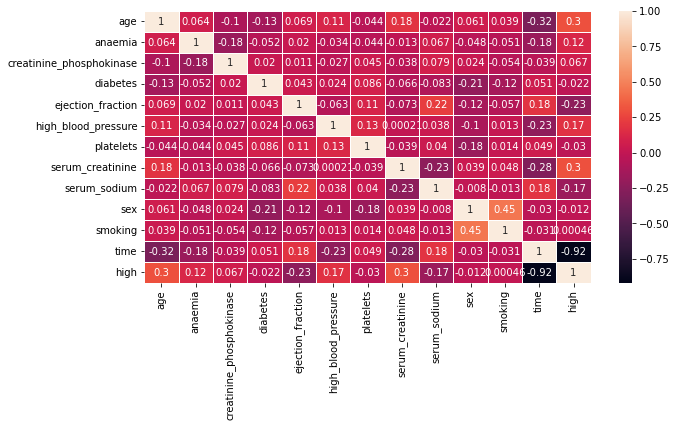
\includegraphics[width=7.5in]{figures/correlation_matrix.png}
	\caption{Correlation Matrix}\label{fig:figures/correlation_matrix.png}
\end{figure}

{From this correlation matrix, we can see that there are not many
significant correlations between the variables. There is a -0.92
correlation between the high and time variables but this is because the
high variable depends on what the time variable is(less than or greater
than 140 days). Otherwise the absolute values of the correlations are
less than 0.45 which indicates that the variables are not correlated to
weakly correlated at all. }

{}

{}

\section{Proposed Methodology}

{Predicting risk of death within heart failure patients is a binary
classification problem. Therefore, models such as feed-forward neural
networks, support vector machines, and naive bayes classifiers can be
used to determine the risk of death for a patient.}

{}

{Once the models were trained, we decided to use the model with the best
performance for an interactive web demo. The model would be written to
persistent storage and made available to anyone via a web front end.
Patients can input their medical information to have the model evaluate
their risk level. Depending on the result, the patient can further
consult with their doctor about the need for a quick follow up
appointment.}

{}

{Because medical information must remain private, we must ensure that
information entered on the model is not stored or used in any way by the
model to inform future results. Therefore, a stateless interactive site
with a disclaimer indicating that all information entered is
confidential is necessary.}

{}

\section{Experimental Results}

\subsection{ANN}

\begin{figure}[H]
	\centering
	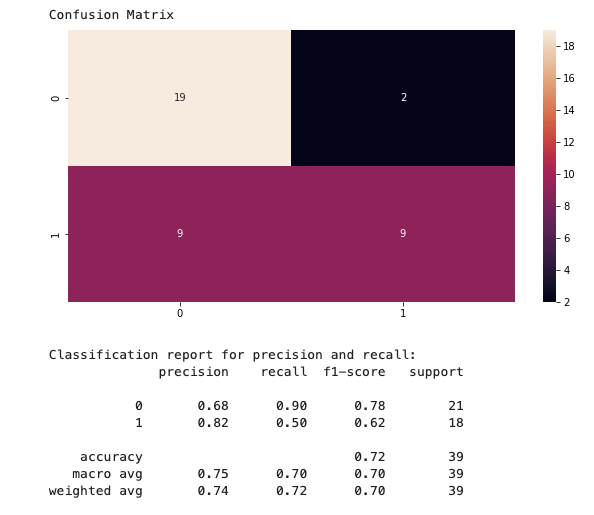
\includegraphics[width=7.5in]{figures/ann_confusion.png}
	\caption{ANN Confusion Matrix}\label{fig:figures/ann_confusion.png}
\end{figure}

{The artificial neural network was built using keras' sequential class.
The original model built included all 12 input features and 2 hidden
layers. The first hidden layer has 12 nodes and the second has 3 nodes.
The activation function for all layers is sigmoid and the number of
epochs for training is 500. For the original model, the testing accuracy
was only 0.513, much lower than 0.703 for the training set. The
difference in accuracy between training and testing sets indicates some
overfitting. This helped improve the updated ANN that we used.}

{}

{For the final ANN, the number of hidden layers was reduced to 1 to
prevent overfitting. We also used a much smaller input feature set, now
only using 4 instead of 12. The features in use are anemia, ejection
fraction, serum\_creatinine, and smoking. In addition, hyperparameters
were manually tuned. The final model uses relu for the hidden layer,
tanh for the output layer, and 1000 epochs for stochastic gradient
descent training. Grid search or random search were not used for
hyperparameter tuning due to a lack of computational resources. However,
manual tuning was able to achieve 0.718 testing accuracy and also
improved the classification metrics by 0.05 to 0.06 in terms of weighted
average. }

{}

\subsection{Naive Bayes Classifier}

\begin{figure}[H]
	\centering
	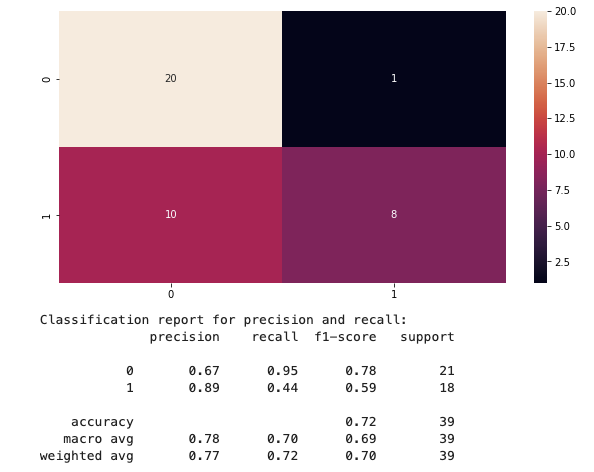
\includegraphics[width=7.5in]{figures/nb_confusion.png}
	\caption{NB Confusion Matrix}\label{fig:figures/nb_confusion.png}
\end{figure}

{The NB classifier was built using GaussianNB from sci-kit learn naive
bayes library. The NB model produced a respectable 0.718 accuracy score
and above 0.70 weighted averages for precision, recall, and f1-score.
However, the model produced a recall of 0.44 for high risk
classification. This means that out of those patients that are truly of
high risk, the model only classified 44\% of them as high risk. This
type of classification problem demands high recall because classifying a
high risk patient as low risk can be fatal. Therefore, the naive bayes
classifier, despite its decent overall performance, was not used.}

{}

\subsection{SVM}

\begin{figure}[H]
	\centering
	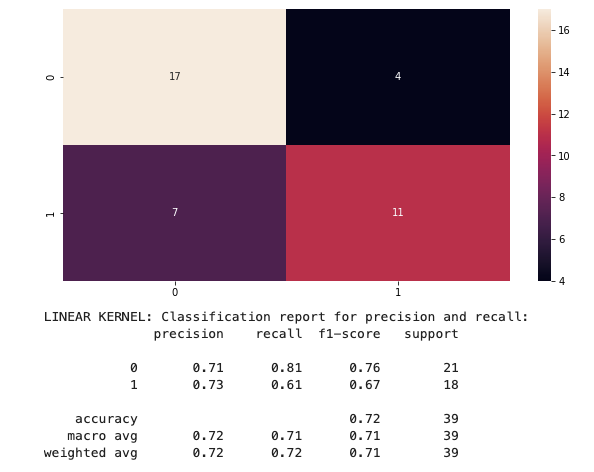
\includegraphics[width=7.5in]{figures/svm_lin_confusion.png}
	\caption{SVM Linear Kernel Confusion Matrix}\label{fig:figures/svm_lin_confusion.png}
\end{figure}

{}

{We built two types of support vector machines using sci-kit learn's SVC
library. Using all 12 input features, the model with the linear kernel
(results above) weighted averages of 0.71 to 0.72 for precision, recall,
and f1-score. However, the recall for high risk classification was
slightly below the average for 0.61, which is very important to this
classification problem. }

\begin{figure}[H]
	\centering
	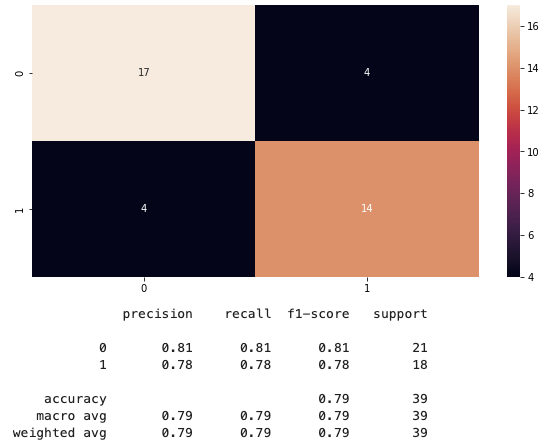
\includegraphics[width=7.5in]{figures/svm_rbf_confusion.png}
	\caption{SVM RBF Kernel Confusion Matrix}\label{fig:figures/svm_rbf_confusion.png}
\end{figure}

{The RBF kernel (results above) performed much better in this regard. It
averaged an accuracy of 0.79 for precision, recall, and f1-score and had
a high risk recall of 0.78. Reducing the input features to the 4 used in
ANN caused a reduction in performance for both kernels. The high risk
recall dropped to 0.33 for linear and 0.44 for RBF. Therefore, the model
with 12 input features and the RBF kernel performed best for SVMs.}

{}

\section{Conclusion and Discussion}

{After constructing artificial neural network, naive bayes', and support
vector machine models, we achieved an accuracy of 0.79 with the SVM RBF
kernel model with all 12 input features. One way the performance of the
models could be improved in the future is to use PCA or t-SNE to reduce
the number of features. This would increase performance during training
and may improve accuracy by removing unnecessary or harmful features. }

{}

\section{Demo}

{Our demonstration shows how our application could be used by medical
professionals when determining whether to discharge a patient with
recent chest pains from the hospital. The program prompts the doctor to
enter the patient's vitals into the cmd line and then the program
responds with a window that shows the patient's name, medical info, and
a recommendation on whether the patient should be released or not. We
know that the command line is not a doctor friendly interface and this
is something that we would address in the future.}

{}

\section{References}

\subsection{Dataset}

\noindent{\href{https://archive.ics.uci.edu/ml/datasets/Heart+failure+clinical+records}{https://archive.ics.uci.edu/ml/datasets/Heart+failure+clinical+records}}

{}

\subsection{Literature review}

\noindent{Davide Chicco, Giuseppe Jurman: "Machine learning can predict survival
of patients with heart failure from serum creatinine and ejection
fraction alone". BMC Medical Informatics and Decision Making 20, 16
(2020).
}{\href{https://bmcmedinformdecismak.biomedcentral.com/articles/10.1186/s12911-020-1023-5}{https://bmcmedinformdecismak.biomedcentral.com/articles/10.1186/s12911-020-1023-5}}{~}

{}

\section{Github}

\noindent{\href{https://github.com/mjpitts/ecs171\_group\_17/}{https://github.com/mjpitts/ecs171\_group\_17/}}
{}

\end{document}
